\documentclass[12pt, letterpaper]{article}
\usepackage[utf8]{inputenc}
\usepackage[document]{ragged2e}
\usepackage{graphicx}
\usepackage{comment}
\usepackage[normalem]{ulem} % for strikethrough text
\usepackage{float} % for passing float parameter into the picture environment
\usepackage{listings}

%\lstdefinestyle{mystyle}{
%	tabsize=0.5,
%	basicstyle=\footnotesize
%}
%\lstset{style=mystyle}

\graphicspath{{images/}}


% from here content will be shown
\begin{document}

\begin{titlepage}
\centering
{\Large DESIGN DOCUMENT} \\
\begin{figure}[H]
\centering

\includegraphics[width=5cm]{Logo_Politecnico_Milano.png}
\caption{Politecnico di Milano}
\label{fig:PoliMi}
\end{figure}
\textbf{version 1.0} \\
\vspace{0.5cm}
Artemiy Frolov, mat. 876373 \\
\vspace{0.5cm}
autumn 2016
\end{titlepage}


\tableofcontents{}

\newpage

\section{Introduction}
\subsection{Purpose}

The purpose of this document is to provide more technical details about the CarSharing System software application.

This document is directed to developers and is necessary to state these aspects of the developing system: 
\begin{itemize}
	\item high level architecture 
	\item runtime view 
	\item choosed architectural styles and patterns
	\item algorithm design of key components 
	\item possibly include some extensions of the user interface defined in RASD 
\end{itemize}

\subsection{Scope}

CarSharing is a web-based software application that helps car-sharing companies to increase usability of their service, by providing more convenient way of renting electric cars for clients via smartphones, hence helping clients to use the service in a more comfortable way. Thus, the software is targed only to:
\begin{itemize}
	\item Users
\end{itemize}    

System allow clients(Users) to locate available electrical cars, with all relevant information about it (inluding current battery fulness, address, registered number) nearby or in the specific area. \\ 
After selecting the car, user can reserve it for up to one hour. When a user reaches the reserved car, system allows the user to unlock the car via button in the web-app. As soon as the engine ignites, the system confirms that the car is now occupied and user can see current charges through the screen in
the car. \\
User can leave the car for a short period of time without missing the car occupation. When the user no more needs the car, he presses the "Stop the trip" button, system locks the car and collect the money from the bank account, provided by user during registration. From this point the car is no more controlled by the user and it be becomes available again. \\
System, in order to restrain the behaviour of users, and to encourage virtuous behaviours of users, carries out some reward and punishment features.
Also the system uses external web-services to present the location of cars on the application website and to manage payments.   

\subsection{Definitions, Acronyms, Abbreviations}

\begin{itemize}
	\item RASD: requirement analysis and specification document 
	\item DD: design document
	\item SMS: short message service; used to notify users 15 minutes before the reservation time expires, also used for a short period suspendance warning. A SMS gateway is needed to use it.
	\item SMS gateway: it is a service which allows to send SMS via standard API.
	\item MVC: model view controller.
	\item REST: REpresentational State Transfer
	\item RESTful: REST without session
	\item API: Application Programming Interface
	\item OS: Operating System
	\item JDO: Java Data Objects
	\item JDOQL: Java Data Object Query Language
\end{itemize}


\subsection{Reference Documents} 

\begin{itemize}
	\item RASD produced before 1.1
	\item Specification Document: Assignments 1 and 2 (RASD and DD).pdf
\end{itemize}

\subsection{Document Structure}

\begin{itemize}
\item Introduction
	\begin{itemize}
		\item Purpose 
		\item Scope
		\item Definitions, Acronyms, Abbreviations
		\item Reference Documents
		\item Document Structure 
	\end{itemize}
\item Architecture Design
	\begin{itemize}
		\item Overview:	High level components and their interaction
		\item Component view
		\item Deployment view
		\item Runtime view: mostly contain sequence diagrams to describe the way components interact
		\item Component	interfaces
		\item Selected architectural styles and	patterns 
		\item Other	design decisions
	\end{itemize}
\item Algorithm Design
\item User Interface Design
\item Requirement Tracebility
\item Effort Spent
\item Reference

\end{itemize}

\newpage
\section{Architectural Design} 
\subsection{Overview}

The CarSharing system would have 3 tier client-server architecture. 

\begin{figure}[H]
\centering
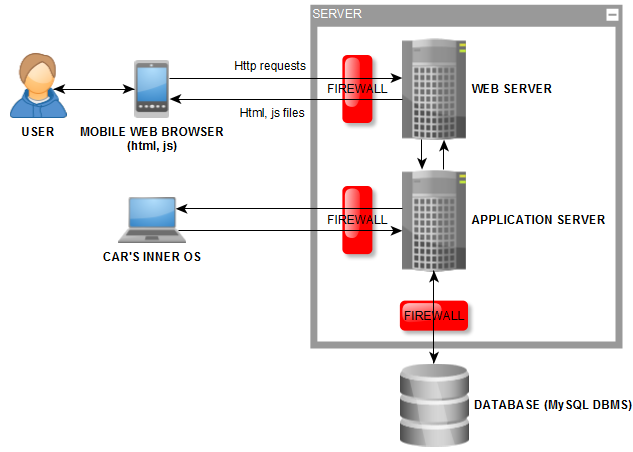
\includegraphics[width=\textwidth]{hlarch.png}
\caption{High-level architecture representation}
\label{fig:hlarch}
\end{figure}

\textbf{Mobile web browser:} browser that user uses on his/her smartphone. \\ 
\vspace{0.5cm}
\textbf{Web server:} Server that provide webpages to client and acquires input data collected from users' webpages. \\
Mobile web browser sends http requests to the web server, which responds by sending proper html and js files. \\
Mobile web browser and web server form the GUI and both correspond to the Presentation tier of the cliet-server high-level architecture. \\
\vspace{0.5cm}
\textbf{Application server:} server that processes the data and manage application logic. \\ 
Application server corresponds to the Logic tier of the cliet-server high-level architecture. \\
\vspace{0.5cm}
\textbf{Car's inner OS:} operating system of the electrical car. \\ 
\vspace{0.5cm}
\textbf{Database:} Persistent data storage. Must be RDBMS. \\
Database corresponds to the Data tier of the cliet-server high-level architecture. \\
\vspace{0.5cm}
Application server receives user's activity information from the web server via RESTful API. Received information is then processed and can be stored in database or/and affect electrical car states. \\
Application server communicates with the electrical car's inner OS via 2G/3G/4G. Cellular network technology can be used. \\
\vspace{0.5cm}

\begin{figure}[H]
\centering
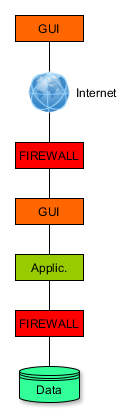
\includegraphics[width=4cm]{tiers.png}
\caption{Tiers}
\label{fig:tiers}
\end{figure}

On the diagram \ref{fig:tiers} tiers are represented. Obviously, that type of tier architecture corresponds to the distributed presentation. \\
From the diagram \ref{fig:tiers} one might notice that there is no firewall between web and application servers. In this architecture assumtion is made, that \underline{web and application logics run on the same server}. But still database can be located apart from logic server, thus firewall is used. 


\subsubsection{High level components and their interactions}

\begin{figure}[H]
\centering
\includegraphics[width=\textwidth]{hlcomponents.png}
\caption{High-level components}
\label{fig:hlcomp}
\end{figure}

\subsection{Component view}

\begin{figure}[H]
\centering
\includegraphics[width=\textwidth]{componentview.png} 
\caption{Components View}
\label{fig:compview}
\end{figure}

\begin{itemize}
	\item RequestController: manages the incomming requests from users and redirect them to system services.
	\item RegistrationController: maintains collected registration information, incuding checking validity of inputed data. 
	\item LogInController: checks if user and password exist in database and connect user to CarSharing services. 
	\item Reservationontroller: manages car reservation. The most important part of the system. It: 
	\begin{itemize}
	   	\item updates reservation status of the car in database.
	   	\item includes backward timer that restricts the time of car reservation during "reserved" status and suspended car during "occupied" status. It provides notification message to NotificationController.  
	   	\item communicates with LocationController(and implicitly with Car) to activate page car control buttons in user's browser and manipulate car's hardware.
	   	\item activates PaymentCalculator to sum up the cost of the ride. 
	\end{itemize}   
	\item NotificationController: sends warning messages to the user about soon expire time of reservation or time of car being suspended via SMS. Has access to the database to acquire telephone number of the user.
	\item LocationController: compares user's and car's locations to enable car controlling features. Communicates with CarController(and implicitly with the Car) to acquire GPS data of the car. Have access to database to acquire general information about the car and provide it to user.  
	\item CarController: Acquires information of the car from sensors, GPS and other relevant information for the CarSharing system. Sends request to the car for manipulation. 
	\item PaymentCalculator: sum up the cost of the ride. Sends requests to the CarController to collect sensors information. Collected information is then transformed into charges and discount of the ride. Has access to the database to collect payment information of the user. Uses external payment web services, sends requests to it with the amount of payment to take and address of the charged bank account. During the ride it continuously calculate current charges and send it to the car to show it on the display.
\end{itemize}

\subsection{Deployment View} 

\begin{figure}[H]
\centering
\includegraphics[width=10cm]{DeploymentView.png} 
\caption{Deployment View}
\label{fig:DepView}
\end{figure}

\newpage
\subsection{Runtime view}
\subsubsection{Defining area of car search}
\begin{figure}[H]
\centering
\includegraphics[width=\textwidth]{3DefAreaOfSearch.png} 
\caption{sequence diagram: Defining area of car search}
\label{fig:3DefAreaOfSearch}
\end{figure}
\newpage
Firstly user chooses where to search cars: nearby user or nearby the specific area provided by user. In the diagram \ref{fig:3DefAreaOfSearch} at the beggining user either presses the button "Nearby" or he/she inputs address into the "Specific area" field and presses button "Submit". In both cases in the diagram these actions are treated as "User\_desired\_area\_of\_car\_search(coord)" and in both cases browser sends coordinates. \\
Then coordinates are transferred to the CarController, which compares coordinates with each available car in the database. It also collects current information about the car, including battery fullness.  If car is not further than 3 (km2) from the coordinates it is added to the set of cars\_nearby. Proccess repeats until all avaiable cars are checked. \\
Then the set of cars\_nearby is sent to external map web service, which is placed in the web page.  
\newpage
\subsubsection{Choosing the car}
\begin{figure}[H]
\centering
\includegraphics[width=\textwidth]{4ChooseCar.png} 
\caption{sequence diagram: Choosing the car}
\label{fig:4ChooseCar}
\end{figure}
\newpage
When user presses on the car on the map the information about it appears near the map window and "reserve" button popes up. When after selecting the car user presses the button "reserve" the system checks the up-to-date information about that car if it is already reserved. If it is not reserved system reserves it for the user(updates the database) and shows the Reservation page.  
\newpage
\subsubsection{Car has been reserved}
\begin{figure}[H]
\centering
\includegraphics[width=\textwidth]{5CarIsReserved1.png} 
\caption{sequence diagram: Car has been reserved}
\label{fig:5CarIsReserved1}
\end{figure}
\newpage
After user reserved the car backward timer is set to 1 hour. Until the timer is not equals to 0 the user can still occupy the car. When user presses the "unlock button" on the web page system checks whether user is close to the car. If not, it return the message "too far from the car to unlock". When users coordinates are close to the coordinates of the car and user presses the "unlock button" the system sends request to the car to unlock itself. At this point when user enters the car and starts the engine, Car sends acknowledgement to the system, ReservationController changes car status to the "occupied", kills the timer and requests the web-application to show the occupation page. \\ 
Note: If the user once unlocked the car, being close to the car, the new validated button "lock" button can be used from any distance. \\
\newpage
\subsubsection{Car has been reserved(continue)}
\begin{figure}[H]
\centering
\includegraphics[width=\textwidth]{6CarIsReserved2.png}
\caption{sequence diagram: Car has been reserved(continue)} 
\label{fig:6CarIsReserved2}
\end{figure}
\newpage
If the timer went to zero and user hasn't started the engine, the system changes car status to "available" and asks the PaymentCalculator to sum up the cost, providing the charge of 1 euro. The error message "reservation is expired" appears in the browser and after few seconds main page is shown.  \\
In the diagram \ref{fig:6CarIsReserved2} the frame "Payment" describes the basic algorithm of the PaymentCalculator. If the addit\_arg is equals to "null", then the algorithm describes the case, when user stops the trip by himself and the step 6 can be ommitted. Also PaymentCalculator methods are described in "Algorithm design" paragraph. \\
In order to restrict the situation when user get into the car, but timer went to 0, system blocks and suspends(if user catched to start it) the car starter and locks the car(not seen in the diagram \ref{fig:6CarIsReserved2}). In that case user can unlock the door from inside, walk off the car and it will automatically lock it again.
\newpage

\subsubsection{Driving charges}
\begin{figure}[H]
\centering
\includegraphics[width=\textwidth]{7DrivingCharges.png} 
\caption{sequence diagram: Driving charges}
\label{fig:7DrivingCharges}
\end{figure}
\newpage

While user is using the car(car is "occupied") the communication between application and car is continuous. ReservationController collects data from car's sensors and check if car's engine is off. In the intermediate step of ReservationController requests this data, PaymentCalculator catches this data, transform this data into the additioning amount of charge to add to the already gained amount(works as "accumulator" of charges) and send it back to the car. Car displays this information on the screen in the car. \\
Once user pressed "End Of Trip" button, communication stops and ReservationController sends request to the PaymentCalculator to form the receipt and send it to the external payment service (this procedure is implemented in the diagram \ref{fig:6CarIsReserved2} in the frame "Payment"). 
\newpage

\subsubsection{Send notification}
\begin{figure}[H]
\centering
\includegraphics[width=\textwidth]{8Notification.png} 
\caption{sequence diagram: Send notification}
\label{fig:8Notification}
\end{figure}
\newpage

This diagram explains both cases when user has only reserved the car, but haven't used it and when the user left the car suspended. Thus, variables "occupied" and "hold" are used to describe both possible cases. Notification only send to the user via SMS, when timer has 15 minutes left. NotificationController uses external services to send SMS to the user. 

\newpage

\subsubsection{Car Is Occupied}
The key feature while user is using the car is described in the diagram \ref{fig:7DrivingCharges}. The runtime diagram for the rest is redundant as it doesn't have any new specific cases that haven't been described yet and mechanisms of implementation are the same. Brief description:
\begin{itemize}
	\item System provides the "Occupied" page, which contains 2 buttons - "lock/unlock" and "End Of Trip"
	\item Procedure of using buttons "lock/unlock" has been described in the runtime diagram \ref{fig:5CarIsReserved1} from the beggining.
	\item Button "End of the Trip" simply sends request to the ReservationController to change car status to "available". After that ReservationController sends request to the CarController to block the car starter(Car also locks itself) and requests the PaymentCalculator to sum up the total cost of the ride(see diagram \ref{fig:6CarIsReserved2} and read the description below).
	\item If user has just left the car suspended, timer again activates and the procedures are repeated as mentioned in the \ref{fig:5CarIsReserved1}, but without request 4.1.1.3 and variable "occupied" must be replaced with "hold" to distinguish situations when user just reserved the car and suspended the car for a while.
\end{itemize}  
\newpage

\subsection{Component interfaces}
\begin{figure}[H]
\centering
\includegraphics[width=\textwidth]{ComponentInterfaces.png} 
\caption{Component Interface}
\label{fig:CompInter}
\end{figure}

\subsection{Selected architectural styles and patterns}
\subsubsection{Overall Architecture}

Application is divided into 3 layers:
\begin{itemize}
	\item [1)] Database (DAL: Data Access Layer)
	\item [2)] Application logic (BLL: Business Logic Layer)
	\item [3)] Thin Client (interface with BLL)
\end{itemize}

\subsubsection{Selected achitectural styles and patterns}

\sout{Architectural style chosen is based on SOA(Service-Oriented Architecture):}
\begin{itemize}
	\item \sout{Service requestor: RequestController}
	\item \sout{Service providers:}
	\begin{itemize}
		\item \sout{RegistrationController}
		\item \sout{LogInController}
		\item \sout{ReservationController}
	\end{itemize}
	\item \sout{Microservices:}
	\begin{itemize}
		\item \sout{CarController}
		\item \sout{NotificationController}
		\item \sout{BackwardTimer}
		\item \sout{PaymentCalculator}
	\end{itemize}
\end{itemize}

\vspace{0.5cm}
\textbf{MVC} \\
\vspace{0.5cm}

Obviously, as in most web applications, Model-View-Controller pattern is used. 
Due to the fact, that Thin Client paradigm is used, View and partly Controller parts will be held on the client side, while the major Controller logic and Model part will be on the Server side.    

\vspace{0.5cm}
\textbf{Client-Server} \\
\vspace{0.5cm}
As in the application design Thin Client paradigm is used, it is necessarily mean that Client-Server pattern must be used. Thus, application is run on the server to decrease requirements from the users' hardware. \\
Client-Server pattern is comfortable in the sense that all users' requests are maintained by the same application on one server. \\
Moreover it is also easy to increase scalability via adding additional clusters to the server, if the number of users gets larger. \\
\newpage

\subsubsection{Protocols}

Protocols that are going to be used are mentioned above. \\

\vspace{0.5cm}
\textbf{JDO(Java Data Objects)} \\
\vspace{0.5cm}

JDO API will be used to implement communication between BLL and DAL. JDO can be easily used along with Java business logic code. \\
Contains JDOQL to run SQL queries to database. \\
Besides, JDO is database independent, which is convenient. From the oracle.com quote: "Applications written with the JDO API are independent of the underlying database. JDO implementations support many different kinds of transactional data stores, including relational and object databases, XML, flat files, and others." \\
Moreover, it has other pros like portability, high performance, ease of use, integration with EJB.

\vspace{0.5cm}
\textbf{RESTful API} \\
\vspace{0.5cm}
RESTful API is used to organize commication between client and BLL via http requests. \\
Commonly used communication protocol used in web-applications.
\vspace{0.5cm}
\textbf{Open IoT Stack for Java} \\
\vspace{0.5cm}
Will be used to send request to the car, control it and acquire data from it. This is a built solution to control IoT devices, can also be used to, quote "configure the network, such as Wi-Fi and cellular bearers, LAN, firewalling and routing, etc".


\section{Algorithm design}
\label{sub:alg_des}
\subsection{PaymentCalculator methods}
In UML sequence diagrams above PaymentCalculator methods are not exposed. \\
In the pseudo-code below the charging step and sum up procedures are described. Charging step is used in the situation, when user uses the car and the charging information is displayed on the creen in the car. Sum up procedure is used after user used "End The Trip" button or lost reservation to calculate the total cost of the ride and use external payment service to implement the payment procedure. \\
Also transformation from sensor information to cost function is described. Other functions used in sumUp and calculateChargingStep are not decribed, but their meanings can be derived from their names.

\begin{lstlisting}[basicstyle=\footnotesize, tabsize=1]
// continues computation to show on display
function calculateChargingStep(User $user) { 
	// charge is static, to accumulate
	static $charge = 0;
	// request to collect sensor information from the user's car
	$car_sens_inf = getCarSensorInfo($user->car);
	// Check other car information
	$
	// accumulate charge
	$charge += transformSensorInfoToCost($car_sens_inf, 0);
	// send $charge to the car's display
	sendToDisplay($charge);
}   
// When user looses the car control (whether by his own will or by loosing reservation)
function sumUp(User $user, Charge $charge, Addit_arg $arg) { 
	if($arg != NULL) {
	// charge for 1 euro 
	$charge += 1;
	}
	// request to collect sensor information from the user's car
	$car_sens_inf = getCarSensorInfo($user->car);
	// compute the total charge
	$charge = transformSensorInfoToCost($car_sens_inf, $charge);
	// get payment address from the DB 
	$payment_address = getUserPaymentAddress($user);
	// Send request to external payment service
	sendPaymentToExternalService($payment_address, $charg);
}

function transformSensorInfoToCost(CarSensInfo $car_sens_inf, Charge $charge) {
	// dicount for 2 passengers
	const disc2pass = 0.9;
	// discount for engine being turned off
	const discEngOff = VALUE1; // value is defined by the company 
	// dicount for 50% energy left after ride
	const disc50energy = 0.8;
	// charge per minute
	const charg_per_minute = VALUE2; // value is defined by the company
	// Mean time between acquiring sensor info from the car and sending charging info 
	// back to the car
	const mean_time; // value must be defined by engineers
	if(getReservationStatus != "available") {
		// Check if user carry 2 more passenger (captured by the camera) 
		if($car_sens_inf->camera->more2passangers->state; == true) {
			$charg = charg_per_minute*mean_time*disc2pass;
		}
		if($car_sens_inf->engine_on == false) {
			$charg = $charg*discEngOff;
		}
		} else {
		if(car_sens_inf->battery > 50) {
			$charge = $charge*disc50energy;
		}
	}
	return $charge;
}


\end{lstlisting}

\newpage
\section{User Interface Design}
\subsection{Mockups}
Mockups have beem already shown in RASD in section 4.2.1.
\subsection{Extensions}
User interface, when user suspends the car and leaves it, is introduced on the picture below.
\begin{figure}[H]
\centering
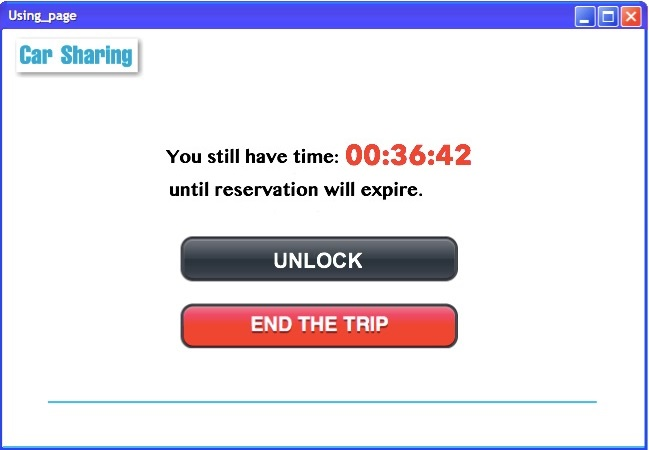
\includegraphics[width=\textwidth]{Extens.jpg} 
\caption{Extension of the "Occupied" webpage, when car is suspended}
\label{fig:Extens}
\end{figure}

\newpage
\section{Requirement traceability}

The aim of the project is to satisfy requirements stated in the RASD.

\begin{itemize}
	\item {[G1]} Registered users(users) can access the system
	\begin{itemize}
		\item RequestController
		\item RegistrationController
		\item LogInController
	\end{itemize}
	\item {[G2]} Users can locate all unoccupied electric cars parked nearby or within a specific area
	\begin{itemize}
		\item RequestController
		\item ReservationController
		\item LocationController
		\item CarController
	\end{itemize}
	\item {[G3]} Users can see the information about battery fulness of each unoccupied electrical car.
	\begin{itemize}
		\item RequestController
		\item ReservationController
		\item LocationController
		\item CarController
	\end{itemize}
	\item {[G4]} Users can reserve available electric car.
	\begin{itemize}
		\item RequestController
		\item ReservationController
	\end{itemize}
	\item {[G5]} Users can access the reserved car
	\begin{itemize}
		\item RequestController
		\item ReservationController
		\item LocationController
		\item CarController
	\end{itemize}
	\item {[G6]} Users can park the car for later usage without missing the "occupied" status.
	\begin{itemize}
		\item RequestController
		\item ReservationController
		\item LocationController
		\item CarController
	\end{itemize}
	\item {[G7]} Users are notified about current driving charges.
	\begin{itemize}
		\item RequestController
		\item ReservationController
		\item PaymentCalculator
		\item CarController
	\end{itemize}
	\item {[G8]} Users are encouraged to use the service properly.
	\item {[G8.1]} Users have a 10\% discount when he picks at least 2 more passenger onto the car.
	\begin{itemize}
		\item RequestController
		\item ReservationController
		\item PaymentCalculator
		\item CarController
		\item + algorithm is described in the paragraph "Algorithm design"
	\end{itemize}
	\item {[G8.2]} Users have a 20\% discount on the ride if he left the car with no more than 50\%
	\begin{itemize}
		\item RequestController
		\item ReservationController
		\item PaymentCalculator
		\item CarController
		\item + algorithm is described in the paragraph "Algorithm design"
	\end{itemize}
\end{itemize}

\newpage
\section {Effort Spent} 
\textbf{Artemiy Frolov:}
\begin{verbatim}
26/11, 1h
28/11, 0.5h
30/11, 3h
1/12, 3h
2/12, 2h
3/12, 3h
4/12, 4h
6/12, 2h
7/12, 2h
8/12, 5h
9/12, 5h
10/12, 2h
11/12, 3h
\end{verbatim} 

\newpage
\section{References}
Used tools \\
The tools we used to create this DD document are:
\begin{itemize}
	\item draw.io: for UML models
	\item Github: for version control
	\item MiKTeX: to compile the DD.tex file to pdf
	\item yEd Graph Editor: for graph and diagrams creation
	\item Pencil: for mockups
\end{itemize}
\newpage


\section{Changelog}
\begin{itemize}
	\item v1.1:
	\begin{itemize}
		\item in the section "Selected architectural styles and patterns", subsection "Overall architecture", word "tiers" changed to "layers".
		\item "Service-oriented paradigm (SOA)" is deleted, as it is not suitable for the current application.  
	\end{itemize}	 	
\end{itemize}

\end{document}